\documentclass{standalone}
\usepackage{tikz}
\usetikzlibrary{patterns, positioning}
\usepackage[sfdefault]{ClearSans} %% option 'sfdefault' activates Clear Sans as the default text font
\usepackage[T1]{fontenc}

\begin{document}
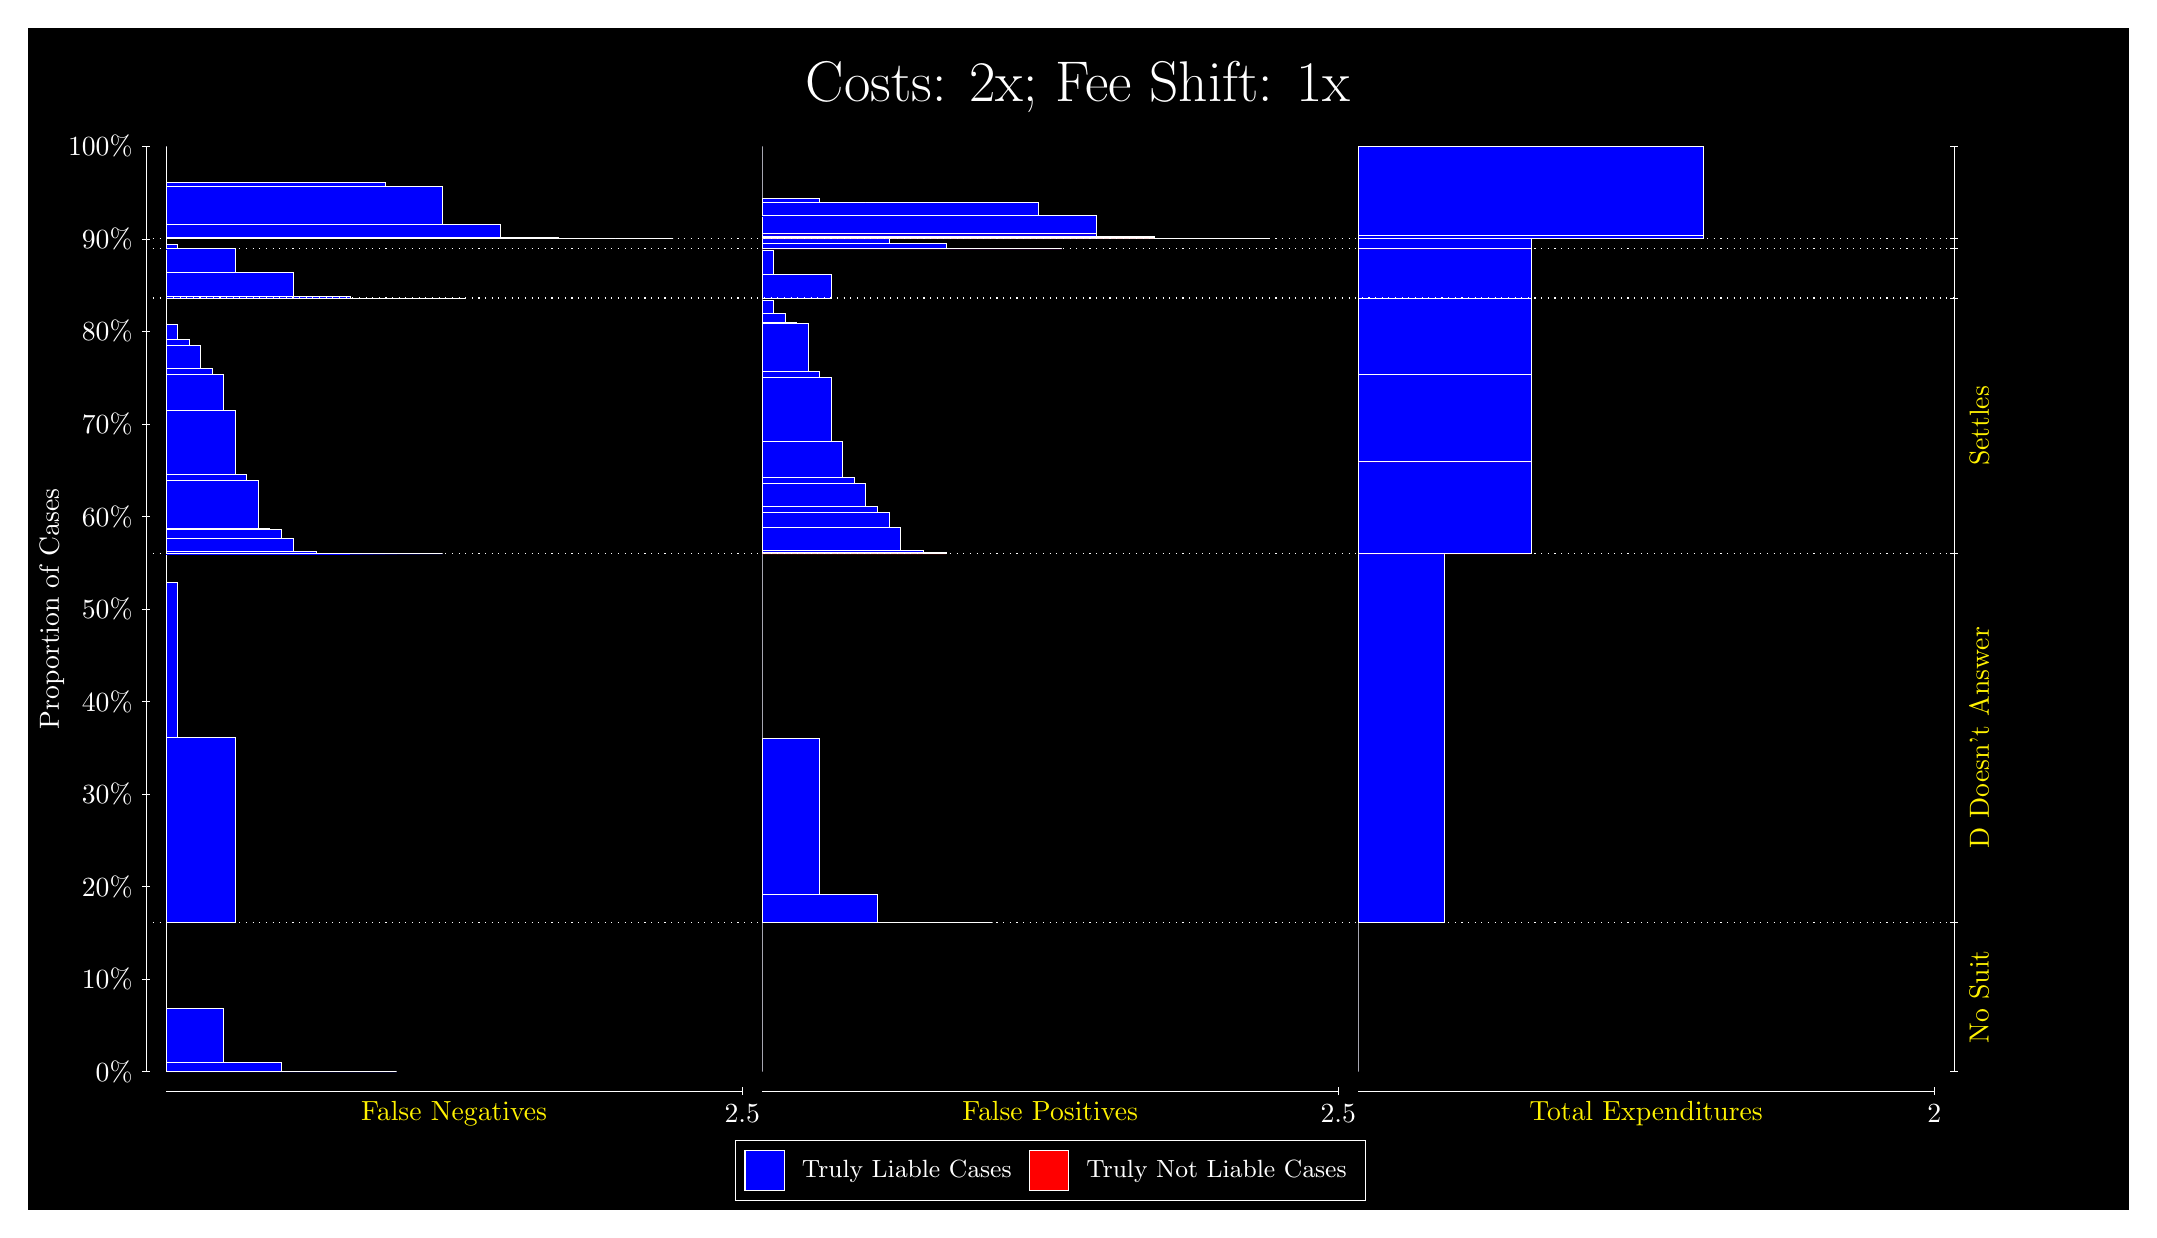
\begin{tikzpicture}
\draw[fill=black] (0,0) rectangle (26.667,15);
\draw[text=white] (0,13.5) rectangle (26.667,15) node[midway] {\huge Costs: 2x; Fee Shift: 1x};
\draw[white, very thin] (1.5,1.75) -- (1.5,13.5);
\node[rotate=90, text=white, anchor=center] at (0.3, 7.625) {Proportion of Cases};
\draw[white, very thin] (1.45,1.75) -- (1.55,1.75);
\node[text=white, anchor=east] at (1.45, 1.75) {0\%};
\draw[white, very thin] (1.45,2.925) -- (1.55,2.925);
\node[text=white, anchor=east] at (1.45, 2.925) {10\%};
\draw[white, very thin] (1.45,4.1) -- (1.55,4.1);
\node[text=white, anchor=east] at (1.45, 4.1) {20\%};
\draw[white, very thin] (1.45,5.275) -- (1.55,5.275);
\node[text=white, anchor=east] at (1.45, 5.275) {30\%};
\draw[white, very thin] (1.45,6.45) -- (1.55,6.45);
\node[text=white, anchor=east] at (1.45, 6.45) {40\%};
\draw[white, very thin] (1.45,7.625) -- (1.55,7.625);
\node[text=white, anchor=east] at (1.45, 7.625) {50\%};
\draw[white, very thin] (1.45,8.8) -- (1.55,8.8);
\node[text=white, anchor=east] at (1.45, 8.8) {60\%};
\draw[white, very thin] (1.45,9.975) -- (1.55,9.975);
\node[text=white, anchor=east] at (1.45, 9.975) {70\%};
\draw[white, very thin] (1.45,11.15) -- (1.55,11.15);
\node[text=white, anchor=east] at (1.45, 11.15) {80\%};
\draw[white, very thin] (1.45,12.325) -- (1.55,12.325);
\node[text=white, anchor=east] at (1.45, 12.325) {90\%};
\draw[white, very thin] (1.45,13.5) -- (1.55,13.5);
\node[text=white, anchor=east] at (1.45, 13.5) {100\%};

\draw[white, very thin] (24.457,1.75) -- (24.457,13.5);
\draw[white, very thin] (24.407,1.75) -- (24.507,1.75);
\node[anchor=west] at (24.407, 1.75) {};
\draw[white, very thin] (24.407,3.6473) -- (24.507,3.6473);
\node[anchor=west] at (24.407, 3.6473) {};
\draw[white, very thin] (24.407,8.3258) -- (24.507,8.3258);
\node[anchor=west] at (24.407, 8.3258) {};
\draw[white, very thin] (24.407,11.574) -- (24.507,11.574);
\node[anchor=west] at (24.407, 11.574) {};
\draw[white, very thin] (24.407,12.2) -- (24.507,12.2);
\node[anchor=west] at (24.407, 12.2) {};
\draw[white, very thin] (24.407,12.335) -- (24.507,12.335);
\node[anchor=west] at (24.407, 12.335) {};
\draw[white, very thin] (24.407,13.5) -- (24.507,13.5);
\node[anchor=west] at (24.407, 13.5) {};

\draw[white, very thin, fill=blue] (1.75,1.75) rectangle (4.6775,1.75);
\draw[white, very thin, fill=blue] (1.75,1.75) rectangle (3.9457,1.751);
\draw[white, very thin, fill=blue] (1.75,1.751) rectangle (3.2138,1.8683);
\draw[white, very thin, fill=blue] (1.75,1.8683) rectangle (2.4819,2.5563);
\draw[white, very thin, fill=red] (1.75,2.5563) rectangle (1.75,2.5563);
\draw[white, very thin, fill=blue] (1.75,2.5563) rectangle (1.75,3.6473);
\draw[white, very thin, fill=blue] (1.75,3.6473) rectangle (2.6283,5.9935);
\draw[white, very thin, fill=blue] (1.75,5.9935) rectangle (1.8964,7.9693);
\draw[white, very thin, fill=red] (1.75,7.9693) rectangle (1.75,7.9693);
\draw[white, very thin, fill=blue] (1.75,7.9693) rectangle (1.75,8.3258);
\draw[white, very thin, fill=blue] (1.75,8.3258) rectangle (5.2631,8.3258);
\draw[white, very thin, fill=blue] (1.75,8.3258) rectangle (4.9703,8.3258);
\draw[white, very thin, fill=blue] (1.75,8.3258) rectangle (4.6775,8.3258);
\draw[white, very thin, fill=blue] (1.75,8.3258) rectangle (4.5312,8.3258);
\draw[white, very thin, fill=blue] (1.75,8.3258) rectangle (4.3848,8.3258);
\draw[white, very thin, fill=blue] (1.75,8.3258) rectangle (4.2384,8.3258);
\draw[white, very thin, fill=blue] (1.75,8.3258) rectangle (4.092,8.3262);
\draw[white, very thin, fill=blue] (1.75,8.3262) rectangle (3.9457,8.3269);
\draw[white, very thin, fill=blue] (1.75,8.3269) rectangle (3.7993,8.3269);
\draw[white, very thin, fill=blue] (1.75,8.3269) rectangle (3.6529,8.3531);
\draw[white, very thin, fill=blue] (1.75,8.3531) rectangle (3.5065,8.3563);
\draw[white, very thin, fill=blue] (1.75,8.3563) rectangle (3.3602,8.5165);
\draw[white, very thin, fill=blue] (1.75,8.5165) rectangle (3.2138,8.6372);
\draw[white, very thin, fill=blue] (1.75,8.6372) rectangle (3.0674,8.6498);
\draw[white, very thin, fill=blue] (1.75,8.6498) rectangle (2.921,9.2623);
\draw[white, very thin, fill=blue] (1.75,9.2623) rectangle (2.7746,9.3352);
\draw[white, very thin, fill=blue] (1.75,9.3352) rectangle (2.6283,10.147);
\draw[white, very thin, fill=blue] (1.75,10.147) rectangle (2.4819,10.608);
\draw[white, very thin, fill=blue] (1.75,10.608) rectangle (2.3355,10.682);
\draw[white, very thin, fill=blue] (1.75,10.682) rectangle (2.1891,10.976);
\draw[white, very thin, fill=blue] (1.75,10.976) rectangle (2.0428,11.049);
\draw[white, very thin, fill=blue] (1.75,11.049) rectangle (1.8964,11.234);
\draw[white, very thin, fill=red] (1.75,11.234) rectangle (1.75,11.234);
\draw[white, very thin, fill=blue] (1.75,11.234) rectangle (1.75,11.574);
\draw[white, very thin, fill=blue] (1.75,11.574) rectangle (5.5558,11.574);
\draw[white, very thin, fill=blue] (1.75,11.574) rectangle (4.8239,11.574);
\draw[white, very thin, fill=blue] (1.75,11.574) rectangle (4.092,11.6);
\draw[white, very thin, fill=blue] (1.75,11.6) rectangle (3.3602,11.899);
\draw[white, very thin, fill=blue] (1.75,11.899) rectangle (2.6283,12.2);
\draw[white, very thin, fill=red] (1.75,12.2) rectangle (1.75,12.2);
\draw[white, very thin, fill=blue] (1.75,12.2) rectangle (2.6283,12.201);
\draw[white, very thin, fill=blue] (1.75,12.201) rectangle (1.8964,12.262);
\draw[white, very thin, fill=red] (1.75,12.262) rectangle (1.75,12.262);
\draw[white, very thin, fill=blue] (1.75,12.262) rectangle (1.75,12.335);
\draw[white, very thin, fill=blue] (1.75,12.335) rectangle (8.1906,12.335);
\draw[white, very thin, fill=blue] (1.75,12.335) rectangle (7.4587,12.335);
\draw[white, very thin, fill=blue] (1.75,12.335) rectangle (6.7268,12.344);
\draw[white, very thin, fill=blue] (1.75,12.344) rectangle (5.9949,12.504);
\draw[white, very thin, fill=blue] (1.75,12.504) rectangle (5.2631,12.991);
\draw[white, very thin, fill=blue] (1.75,12.991) rectangle (4.5312,13.041);
\draw[white, very thin, fill=blue] (1.75,13.041) rectangle (3.9457,13.041);
\draw[white, very thin, fill=blue] (1.75,13.041) rectangle (3.7993,13.041);
\draw[white, very thin, fill=blue] (1.75,13.041) rectangle (3.2138,13.041);
\draw[white, very thin, fill=blue] (1.75,13.041) rectangle (2.4819,13.043);
\draw[white, very thin, fill=red] (1.75,13.043) rectangle (1.75,13.043);
\draw[white, very thin, fill=blue] (1.75,13.043) rectangle (1.75,13.5);
\draw[white, very thin, fill=red] (9.3189,1.75) rectangle (9.3189,1.75);
\draw[white, very thin, fill=blue] (9.3189,1.75) rectangle (9.3189,3.6473);
\draw[white, very thin, fill=red] (9.3189,3.6473) rectangle (12.246,3.6473);
\draw[white, very thin, fill=blue] (9.3189,3.6473) rectangle (12.246,3.6473);
\draw[white, very thin, fill=blue] (9.3189,3.6473) rectangle (11.515,3.6496);
\draw[white, very thin, fill=blue] (9.3189,3.6496) rectangle (10.783,4.0038);
\draw[white, very thin, fill=blue] (9.3189,4.0038) rectangle (10.051,5.9796);
\draw[white, very thin, fill=blue] (9.3189,5.9796) rectangle (9.3189,8.3258);
\draw[white, very thin, fill=red] (9.3189,8.3258) rectangle (11.661,8.3258);
\draw[white, very thin, fill=blue] (9.3189,8.3258) rectangle (11.661,8.3384);
\draw[white, very thin, fill=red] (9.3189,8.3384) rectangle (11.368,8.3384);
\draw[white, very thin, fill=blue] (9.3189,8.3384) rectangle (11.368,8.3761);
\draw[white, very thin, fill=red] (9.3189,8.3761) rectangle (11.075,8.3761);
\draw[white, very thin, fill=blue] (9.3189,8.3761) rectangle (11.075,8.6653);
\draw[white, very thin, fill=blue] (9.3189,8.6653) rectangle (10.929,8.851);
\draw[white, very thin, fill=red] (9.3189,8.851) rectangle (10.783,8.851);
\draw[white, very thin, fill=blue] (9.3189,8.851) rectangle (10.783,8.9242);
\draw[white, very thin, fill=blue] (9.3189,8.9242) rectangle (10.636,9.2183);
\draw[white, very thin, fill=red] (9.3189,9.2183) rectangle (10.49,9.2183);
\draw[white, very thin, fill=blue] (9.3189,9.2183) rectangle (10.49,9.2914);
\draw[white, very thin, fill=blue] (9.3189,9.2914) rectangle (10.344,9.7524);
\draw[white, very thin, fill=blue] (9.3189,9.7524) rectangle (10.197,10.565);
\draw[white, very thin, fill=blue] (9.3189,10.565) rectangle (10.051,10.637);
\draw[white, very thin, fill=blue] (9.3189,10.637) rectangle (9.9044,11.25);
\draw[white, very thin, fill=blue] (9.3189,11.25) rectangle (9.758,11.263);
\draw[white, very thin, fill=blue] (9.3189,11.263) rectangle (9.6116,11.383);
\draw[white, very thin, fill=blue] (9.3189,11.383) rectangle (9.4652,11.543);
\draw[white, very thin, fill=blue] (9.3189,11.543) rectangle (9.3189,11.574);
\draw[white, very thin, fill=red] (9.3189,11.574) rectangle (10.197,11.574);
\draw[white, very thin, fill=blue] (9.3189,11.574) rectangle (10.197,11.875);
\draw[white, very thin, fill=blue] (9.3189,11.875) rectangle (9.4652,12.174);
\draw[white, very thin, fill=blue] (9.3189,12.174) rectangle (9.3189,12.2);
\draw[white, very thin, fill=red] (9.3189,12.2) rectangle (13.125,12.2);
\draw[white, very thin, fill=blue] (9.3189,12.2) rectangle (13.125,12.2);
\draw[white, very thin, fill=blue] (9.3189,12.2) rectangle (12.393,12.211);
\draw[white, very thin, fill=blue] (9.3189,12.211) rectangle (11.661,12.273);
\draw[white, very thin, fill=blue] (9.3189,12.273) rectangle (10.929,12.334);
\draw[white, very thin, fill=blue] (9.3189,12.334) rectangle (10.197,12.335);
\draw[white, very thin, fill=red] (9.3189,12.335) rectangle (15.759,12.335);
\draw[white, very thin, fill=blue] (9.3189,12.335) rectangle (15.759,12.335);
\draw[white, very thin, fill=blue] (9.3189,12.335) rectangle (15.028,12.335);
\draw[white, very thin, fill=red] (9.3189,12.335) rectangle (15.028,12.335);
\draw[white, very thin, fill=blue] (9.3189,12.335) rectangle (15.028,12.336);
\draw[white, very thin, fill=blue] (9.3189,12.336) rectangle (14.296,12.341);
\draw[white, very thin, fill=red] (9.3189,12.341) rectangle (14.296,12.341);
\draw[white, very thin, fill=blue] (9.3189,12.341) rectangle (14.296,12.362);
\draw[white, very thin, fill=blue] (9.3189,12.362) rectangle (13.564,12.392);
\draw[white, very thin, fill=red] (9.3189,12.392) rectangle (13.564,12.392);
\draw[white, very thin, fill=blue] (9.3189,12.392) rectangle (13.564,12.619);
\draw[white, very thin, fill=blue] (9.3189,12.619) rectangle (12.832,12.62);
\draw[white, very thin, fill=blue] (9.3189,12.62) rectangle (12.832,12.792);
\draw[white, very thin, fill=blue] (9.3189,12.792) rectangle (12.1,12.794);
\draw[white, very thin, fill=blue] (9.3189,12.794) rectangle (11.368,12.794);
\draw[white, very thin, fill=red] (9.3189,12.794) rectangle (10.783,12.794);
\draw[white, very thin, fill=blue] (9.3189,12.794) rectangle (10.783,12.794);
\draw[white, very thin, fill=blue] (9.3189,12.794) rectangle (10.636,12.794);
\draw[white, very thin, fill=red] (9.3189,12.794) rectangle (10.051,12.794);
\draw[white, very thin, fill=blue] (9.3189,12.794) rectangle (10.051,12.844);
\draw[white, very thin, fill=red] (9.3189,12.844) rectangle (9.3189,12.844);
\draw[white, very thin, fill=blue] (9.3189,12.844) rectangle (9.3189,13.5);
\draw[white, very thin, fill=red] (16.888,1.75) rectangle (16.888,1.75);
\draw[white, very thin, fill=blue] (16.888,1.75) rectangle (16.888,3.6473);
\draw[white, very thin, fill=red] (16.888,3.6473) rectangle (17.986,3.6473);
\draw[white, very thin, fill=blue] (16.888,3.6473) rectangle (17.986,8.3258);
\draw[white, very thin, fill=red] (16.888,8.3258) rectangle (19.083,8.3258);
\draw[white, very thin, fill=blue] (16.888,8.3258) rectangle (19.083,9.4968);
\draw[white, very thin, fill=red] (16.888,9.4968) rectangle (19.083,9.4968);
\draw[white, very thin, fill=blue] (16.888,9.4968) rectangle (19.083,10.603);
\draw[white, very thin, fill=red] (16.888,10.603) rectangle (19.083,10.603);
\draw[white, very thin, fill=blue] (16.888,10.603) rectangle (19.083,11.574);
\draw[white, very thin, fill=red] (16.888,11.574) rectangle (19.083,11.574);
\draw[white, very thin, fill=blue] (16.888,11.574) rectangle (19.083,12.2);
\draw[white, very thin, fill=red] (16.888,12.2) rectangle (19.083,12.2);
\draw[white, very thin, fill=blue] (16.888,12.2) rectangle (19.083,12.335);
\draw[white, very thin, fill=red] (16.888,12.335) rectangle (21.279,12.335);
\draw[white, very thin, fill=blue] (16.888,12.335) rectangle (21.279,12.372);
\draw[white, very thin, fill=red] (16.888,12.372) rectangle (21.279,12.372);
\draw[white, very thin, fill=blue] (16.888,12.372) rectangle (21.279,13.5);
\draw[white, dotted] (1.5,3.6473) -- (24.457,3.6473);
\draw[white, dotted] (1.5,8.3258) -- (24.457,8.3258);
\draw[white, dotted] (1.5,11.574) -- (24.457,11.574);
\draw[white, dotted] (1.5,12.2) -- (24.457,12.2);
\draw[white, dotted] (1.5,12.335) -- (24.457,12.335);
\draw[white, very thin] (1.75,1.5) -- (9.0689,1.5);
\node[text=yellow, anchor=north] at (5.4094, 1.5) {False Negatives};
\draw[white, very thin] (9.0689,1.45) -- (9.0689,1.55);
\node[text=white, anchor=north] at (9.0689, 1.45) {2.5};

\draw[white, very thin] (9.3189,1.5) -- (16.638,1.5);
\node[text=yellow, anchor=north] at (12.978, 1.5) {False Positives};
\draw[white, very thin] (16.638,1.45) -- (16.638,1.55);
\node[text=white, anchor=north] at (16.638, 1.45) {2.5};

\draw[white, very thin] (16.888,1.5) -- (24.207,1.5);
\node[text=yellow, anchor=north] at (20.547, 1.5) {Total Expenditures};
\draw[white, very thin] (24.207,1.45) -- (24.207,1.55);
\node[text=white, anchor=north] at (24.207, 1.45) {2};

\node[text=yellow, centered, rotate=90] at (24.777, 2.6987) {No Suit};
\node[text=yellow, centered, rotate=90] at (24.777, 5.9865) {D Doesn't Answer};
\node[text=yellow, centered, rotate=90] at (24.777, 9.9499) {Settles};




\draw (12.978300999999998,1.5) node[draw=none] (baseCoordinate) {};
\begin{scope}[align=center]
        \matrix[scale=0.5, draw=white, below=0.5cm of baseCoordinate, nodes={draw}, column sep=0.1cm]{
            \node[rectangle, draw, minimum width=0.5cm, minimum height=0.5cm, fill=blue] {}; &
            \node[draw=none, font=\small, text=white] (B) {Truly Liable Cases}; &
            \node[rectangle, draw, minimum width=0.5cm, minimum height=0.5cm, fill=red] {}; &
            \node[draw=none, font=\small, text=white] (B) {Truly Not Liable Cases}; \\
            };
\end{scope}

\end{tikzpicture}
\end{document}